\documentclass[conference]{IEEEtran}
\usepackage[T1]{fontenc}
\usepackage{graphicx}
\usepackage{booktabs}
\usepackage{amsmath}
\usepackage{listings}
\usepackage{xcolor}
\usepackage{url}
\usepackage{cite}
\graphicspath{{../figures/}}
\lstset{basicstyle=\ttfamily\scriptsize, columns=fullflexible, keepspaces=true, showstringspaces=false,
  language=Python, frame=single, framerule=0.3pt, xleftmargin=2pt, xrightmargin=2pt, breaklines=true}
\newcommand{\x}{$\times$}

\begin{document}

\title{Teaching a 4B Gemma to Write TPU Kernels:\\ LoRA Fine-Tuning on Oracle-Verified Pallas Code}

\author{\IEEEauthorblockN{Karthik Vattem, Hruday N., Aarav A.}
\IEEEauthorblockA{Rough draft, November 12, 2026. Author names and affiliations to be completed.}}

\maketitle

\begin{abstract}
Pallas is the kernel language of JAX for Google TPUs. A well written Pallas kernel can outrun the XLA compiler, but the language
is young and thinly documented, and general-purpose language models rarely produce a kernel that compiles. We ask whether
Gemma 4 E4B, a 4-billion-parameter open model, can learn to write Pallas kernels from verified examples alone. We build a TPU
oracle that accepts a solution only if it is a genuine kernel, runs at full size on a TPU v6e, matches a float32 reference on
three seeds, and reaches at least 0.7\x{} the speed of XLA. With it we assemble 2,304 training conversations whose targets were
all judged correct on the chip, written by an open-weights teacher model and a template generator, and we train a rank-64 LoRA
adapter. On the 58-task primary set of JAXBench, with three attempts per task, the base model passes no task with or without
25k tokens of Pallas documentation in its prompt. The adapter passes 9 (exact McNemar $p = 0.004$), which is statistically
indistinguishable from the 7 passed by Gemini Flash with the same documentation ($p = 0.79$). The two models succeed in different
ways: Flash writes a numerically correct kernel for 36 tasks but only 7 are fast enough, whereas the adapter is correct on 9 and
all 9 run faster than XLA (1.30\x{} to 1.39\x{}). Eight of the nine are tiled matrix-multiply kernels, the family our training
data targets at the benchmark's scale, and the skill does not yet extend to array sizes that the learned tiles do not divide.
\end{abstract}

\begin{IEEEkeywords}
code generation, fine-tuning, LoRA, accelerator kernels, TPU, Pallas, JAX, benchmark evaluation
\end{IEEEkeywords}

\section{Introduction}

Most numerical code that runs on an accelerator is compiled automatically. In JAX, a function is traced and handed to XLA,
which chooses how to schedule each operation on the device \cite{jax,mlir}. Decades of work on tensor compilers and schedule search \cite{halide,tvm,ansor} have narrowed the gap to hand-written code without closing it. When the automatic result is not fast enough, an expert
writes a kernel by hand. On Google TPUs \cite{tpu} this is done in Pallas, a JAX extension in which the programmer states how arrays are
cut into blocks, which blocks are loaded into the chip's small fast memory (VMEM) at each step, and what is computed on
them \cite{pallas}. A good kernel keeps the matrix unit busy, never asks for more VMEM than exists, and fuses operations that
XLA would run as separate passes over memory.

Writing such kernels is specialist work. Language models trained on code \cite{codex,alphacode,codellama,starcoder} write ordinary programs well, but they write kernels poorly. Pallas has little public code, its lowering rules for
TPU are strict, and an error in a block shape is only discovered on the chip. JAXBench \cite{jaxbench} measures this directly:
it gives a model a plain JAX function and asks for an equivalent Pallas kernel. Its authors report that most failed samples are
API misuse or compile errors, and they name fine-tuning on curated Pallas corpora as future work. For GPUs, the analogous
problem has received a benchmark \cite{kernelbench} and several trained models \cite{kernelllm,autotriton,kevin}. To our
knowledge no fine-tuned Pallas model has been published, and no result on JAXBench exists for a small open model.

This paper tests whether a small model can acquire the skill through its weights. We fine-tune Gemma 4 E4B \cite{gemma4} with
LoRA \cite{lora}, in the manner of distillation from a stronger teacher \cite{distill}, and compare it with the same model given an identical prompt, so that any difference is attributable to the
adapter. We deliberately give the fine-tuned model no documentation or examples in its prompt. As a reference point we also run
a much larger commercial model, Gemini Flash, with documentation.

Our contributions are as follows.
\begin{itemize}
\item A TPU oracle with a static kernel check, full-size execution, three-seed correctness and a speed bar, used unchanged
for both training-data admission and evaluation (Section~\ref{sec:oracle}).
\item A training set of 2,304 conversations in which every target kernel was judged correct on a TPU, built without any
closed-model output, and screened against the benchmark at the level of the computation rather than the text
(Sections~\ref{sec:contam} and \ref{sec:data}).
\item A serving finding: an adapter that will be served on 4-bit weights must be trained on, and folded into, those exact
quantized weights (Section~\ref{sec:train}).
\item An evaluation in which the adapter raises the base model from 0 to 9 of 58 JAXBench tasks, matching Gemini Flash with
documentation on the pass metric, together with an account of what the adapter did and did not learn
(Sections~\ref{sec:results} and \ref{sec:limits}).
\end{itemize}

\begin{figure*}[t]
\centering
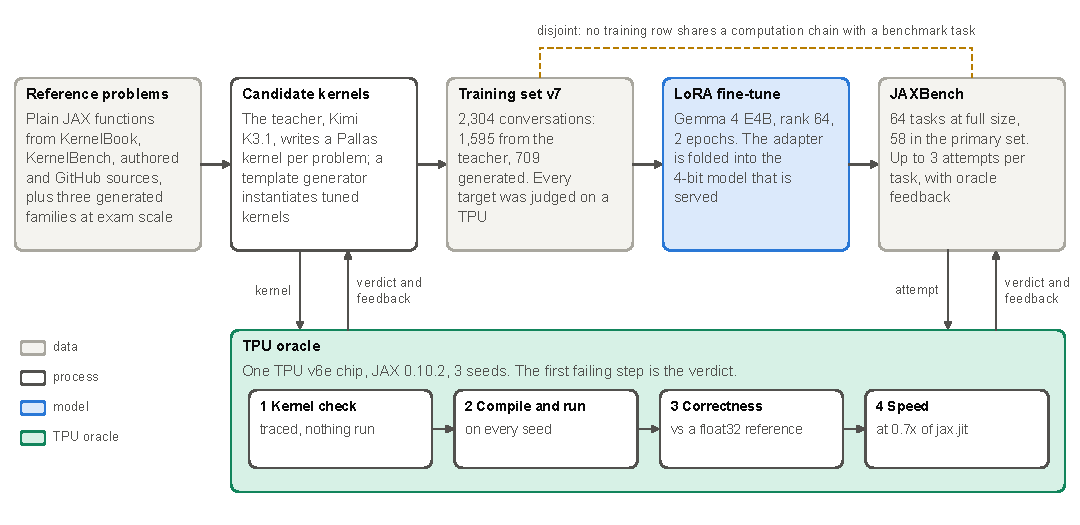
\includegraphics[width=0.92\textwidth]{fig01_overview.pdf}
\caption{Overview. Training targets come from two sources, both judged on a TPU. A LoRA adapter is trained on Gemma 4 E4B, and
the same oracle scores the fine-tuned model on JAXBench.}
\label{fig:overview}
\end{figure*}

\section{Related Work}

\textbf{Kernel benchmarks.} KernelBench \cite{kernelbench} asks models to rewrite PyTorch modules as fast CUDA kernels and
scores correctness and speedup. Follow-up work on verified variants of that benchmark showed that weak tests allow models to
score by exploiting the checker rather than by solving the task \cite{kbverified}. JAXBench \cite{jaxbench} carries the idea to
TPUs: its level 1 contains 50 workloads, 33 operator chains ported from KernelBench (k-tasks) and 17 production kernels such as
attention variants and normalizations (p-tasks). Its authors report that with curated documentation and iterative refinement of
up to 144 attempts per task, a frontier model solves 48 of the 50. None of these works trains a model. Related benchmarks measure whether models can make existing programs faster \cite{pie} or resolve real software issues \cite{swebench}, and learned search has found faster low-level routines than human experts in narrow domains \cite{alphadev}.

\textbf{Trained kernel models.} KernelLLM \cite{kernelllm} fine-tunes an 8B Llama model on PyTorch-to-Triton pairs.
AutoTriton \cite{autotriton}, TritonRL \cite{tritonrl}, Dr.~Kernel \cite{drkernel} and Kevin \cite{kevin} add reinforcement
learning from execution feedback, all for GPUs, where Triton \cite{triton} plays the role that Pallas plays on TPUs. Several of them add guards against reward hacking; the static kernel check in
our oracle plays that role for TPUs.

\textbf{Parameter-efficient fine-tuning.} LoRA \cite{lora} trains low-rank updates to frozen weight matrices, and QLoRA \cite{qlora} trains them over a quantized base. We use LoRA unchanged on a base released with quantization-aware training \cite{qat}.

\textbf{Execution feedback.} Showing a model the error from its own failed program and asking for a correction is an established technique \cite{selfdebug}. Our repair turns and repair training rows follow it, with the TPU oracle as the source of feedback. The only departure from common practice is where the update is applied, which Section~\ref{sec:train} explains.

\section{Method}

\subsection{Task format}

A task is a plain JAX module in the JAXBench layout. A dictionary \texttt{CONFIG} holds every size, \texttt{create\_inputs()}
returns seeded arrays, and \texttt{workload(*inputs)} is the reference computation. A solution is a module that defines
\texttt{workload} with the same arguments and performs its main computation inside \texttt{pl.pallas\_call}.

\subsection{The TPU oracle}
\label{sec:oracle}

Every solution in this paper, whether a candidate training target or a benchmark attempt, is judged by one program
(Fig.~\ref{fig:oracle}). It applies four tests in order and reports the first failure.

\emph{Kernel check.} The solution is traced without being run. It must contain a \texttt{pallas\_call}, the output must depend
on that call, and outside the call only layout and dtype primitives and small integer metadata are allowed. A solution that
computes the answer in ordinary JAX and wraps a token kernel around it is rejected as \texttt{not\_a\_kernel}. This test is
static, so it gives the same verdict on a CPU.

\emph{Execution.} The solution is compiled and run on a TPU v6e at the task's full size. Failures are reported as
\texttt{compile}, \texttt{vmem} (the blocks do not fit on-chip memory), \texttt{mosaic} (the TPU backend rejects the kernel),
\texttt{timeout} or \texttt{runtime}, with the chip's error text.

\emph{Correctness.} The output is compared on three input seeds with a float32 reference computed at the highest matmul
precision. It must agree to absolute and relative tolerance $10^{-2}$, or have at most twice the error that XLA's own compiled
reference has. Otherwise the verdict is \texttt{wrong}.

\emph{Speed.} Let $t_{\mathrm{xla}}$ and $t_{\mathrm{kernel}}$ be the medians of 20 timed calls of the jitted reference and of
the kernel. A correct kernel with $t_{\mathrm{xla}} / t_{\mathrm{kernel}} \ge 0.7$ receives \texttt{pass}; a correct but slower
one receives \texttt{correct\_slow}. The bar of 0.7 is a policy choice: it demands a kernel that is competitive with the
compiler without requiring that a first attempt beat it.

All results use the same oracle files (hash \texttt{c9a07d9298a1}), JAX 0.10.2 and a single v6e chip. Some faulty kernels halt
the TPU core, after which every later item in the same process fails. Our harness re-runs those later items in a fresh process
and never records the collateral failures as verdicts.

\begin{figure}[t]
\centering
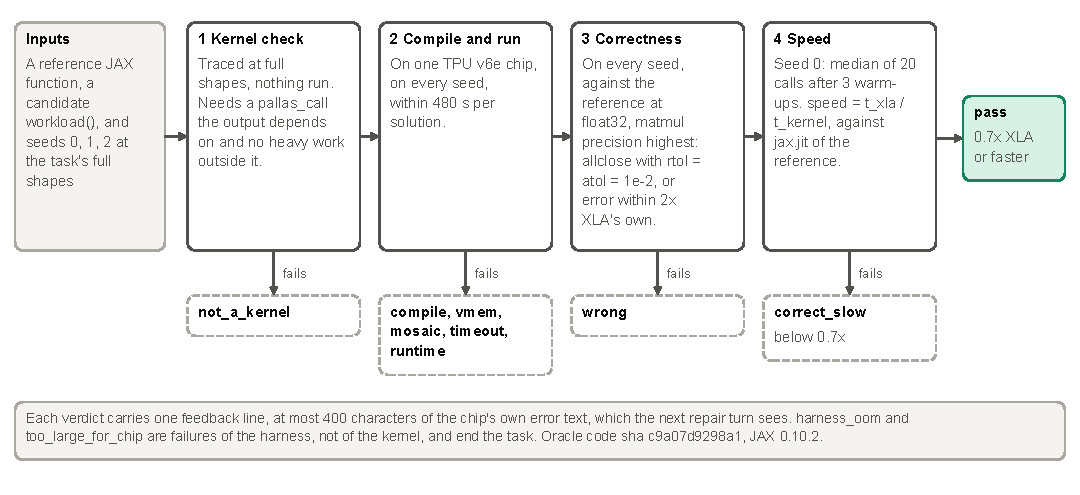
\includegraphics[width=\columnwidth]{fig03_tpu_oracle.pdf}
\caption{The oracle's four tests and the verdict each failure produces.}
\label{fig:oracle}
\end{figure}

\subsection{Source problems and contamination control}
\label{sec:contam}

Training problems come from four places: KernelBench levels 1 and 2 and the KernelBook collection, both ported from PyTorch to
JAX and checked numerically against the original module; operators written for this project, including attention variants,
mixture-of-experts routing, quantized matmuls and state-space scans; and JAX references for publicly available Pallas kernels.
Each problem must pass CPU checks at full size before use: it loads, fits device memory, is deterministic for a seed, varies
across seeds and produces finite output.

JAXBench is used only as an exam. Because JAXBench's k-tasks were themselves ported from KernelBench, a text filter is not
enough to keep exam content out of training, and we exclude a training problem when it is the same kernel as any of the 73
JAXBench files under three tests. The first removes copies: KernelBench problems that JAXBench ported, and near-duplicate
text measured on two token streams. The second compares computations. We trace each \texttt{workload} to JAX's intermediate
representation, reduce it to its chain of primitives, set aside linear arithmetic and layout operations, and exclude the
problem if the remaining chain equals that of a k-task. A problem that cannot be placed with confidence is excluded. The third
is a manual adversarial review of 273 problems that an earlier and coarser rule had excluded by algorithm family; it re-admitted
191 and kept 82 out.

Three independently written checkers confirm on the final file that no excluded problem is present, that no generated row has
an exam chain, and that no JAXBench task name appears. As a text-level check, the training reference closest to any JAXBench
reference has a line similarity of 0.31, whereas JAXBench references resemble each other with a median of 0.66. We stress that
this rule excludes identical computations, not similar ones. Section~\ref{sec:limits} quantifies how close the remaining
training rows are to the tasks the adapter passes.

\subsection{Training data}
\label{sec:data}

A training row is a conversation rendered by the evaluation harness's own prompt function, so the model sees byte-identical
formatting in training and at test time. The target is always a kernel that the oracle judged correct on a TPU. Teacher
reasoning is never a target. A repair row contains the problem, one or two failed kernels with the oracle's verbatim feedback,
and the kernel that finally passed; the loss is computed on the final kernel only, so failed kernels serve as context.

\textbf{Teacher.} Kimi K3.1 \cite{kimi}, an open-weights model, wrote kernels for 1,672 problems from a fixed prompt
containing kernel rules and about 25k tokens of Pallas documentation. On first attempts judged on the TPU, 434 passed and 267
were correct but slow. A second round, prompted with the earlier kernels and the oracle's feedback, added 235 passing problems,
and a third round on 486 problems that had failed twice added 103. No closed-model output is used as a training target.

\textbf{Rows at the benchmark's scale.} An adapter trained on teacher rows alone failed the benchmark's matmul tasks in a
consistent way: it loaded the whole weight into VMEM. The cause was a scale mismatch. The teacher's matmul problems had a
median weight of 2~MB, for which loading the weight whole is correct, while JAXBench's matmul tasks use weights of 268~MB, for
which it overflows. We therefore added rows at production scale in three ways. First, we enlarged 198 matmul-dominant problems
until the weight was at least 64~MB and re-ran their existing kernels; 50 still passed. Second, the teacher repaired the others
using the oracle's feedback and a tiling policy that we measured on the TPU (Fig.~\ref{fig:sweep}): a VMEM limit of 124~MiB and
tiles of $(2048, 2048, 1024)$ along the output rows, output columns and contraction axis. Third, a template generator emits
matmul, batched-matmul and row-reduction kernels that follow the same policy with varied elementwise epilogues, input layouts
and sizes. Of 453 generated candidates judged at full size on the TPU, 434 passed. Nearly every generated row appears a second
time as a surface variant with renamed arguments, configuration keys and docstring, admitted only when its syntax tree equals
the judged kernel's after renaming; a stratified sample of 91 variants passed the oracle 91 of 91.

\begin{figure}[t]
\centering
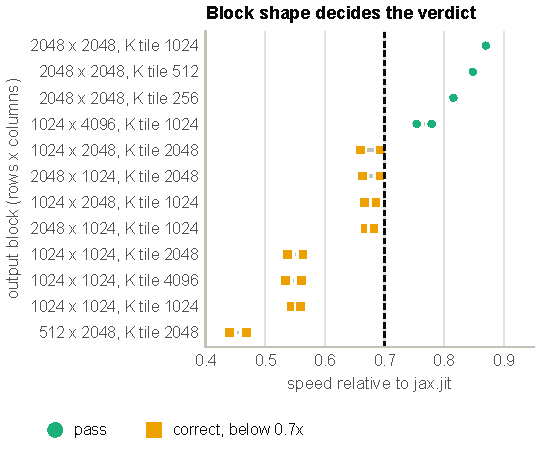
\includegraphics[width=\columnwidth]{fig09_tile_sweep.pdf}
\caption{The TPU sweep behind the tiling policy, for a matmul with 2,048 output rows. Only large output blocks clear the 0.7\x{}
bar; the same kernel with smaller blocks is correct but too slow.}
\label{fig:sweep}
\end{figure}

\textbf{Composition.} Table~\ref{tab:data} gives the final file. The teacher wrote 1,595 targets and the generator 709 (30.8\%).
There are 1,720 single-turn rows and 584 repair chains. For 348 rows (15\%), all on non-matmul teacher problems, the target is
correct but below the speed bar; slow matmul targets were removed because they demonstrate the untiled design that the
production-scale rows are meant to replace. The longest row is 11,854 tokens.

\begin{table}[t]
\caption{Composition of the training set.}
\label{tab:data}
\centering
\begin{tabular}{@{}lr@{}}
\toprule
Part & Rows \\
\midrule
Teacher base set, after contamination filtering & 1,172 \\
Teacher kernels at production scale & 217 \\
Teacher third-round kernels (repair and single-turn) & 206 \\
Template rows (originals and surface variants) & 709 \\
\midrule
Total & 2,304 \\
\bottomrule
\end{tabular}
\end{table}

\subsection{Training and serving}
\label{sec:train}

We train a LoRA adapter of rank 64 and scale 128 on the attention and MLP projections of Gemma 4 E4B (139.5M trainable
parameters), for 2 epochs at a peak learning rate of $10^{-4}$ with AdamW \cite{adamw}, 10\% warm-up, cosine decay and gradient accumulation
of 4, which gives 1,152 optimizer steps. Training took 89 minutes on one A100 80~GB and cost under 6 US dollars. The mean
training loss was 0.157 in the first epoch and 0.075 in the second. The scored checkpoint, the end of epoch 2, was fixed before
training began.

The baselines run the official 4-bit quantization-aware GGUF build of the model under Ollama, which cannot load a LoRA adapter
at run time, so the adapter has to be folded into the weights. In our first attempts we trained on the bf16 weights and
re-quantized the sum to 4 bits. This erased most of the adapter, because typical LoRA updates are far smaller than one 4-bit
rounding step. Two changes fix it. We train against the dequantized 4-bit weights, so that the adapter is fitted to exactly the
base it will be served with, and we store the 258 adapted tensors at 8 bits as the dequantized base plus the update, leaving
every other tensor byte-identical to the official file. The trainer's and the server's token counts agree on all 64 first-turn
prompts, and every evaluation row records the digest of the served model.

\subsection{Evaluation protocol}

\textbf{Tasks.} We use JAXBench's 50 level-1 tasks and 14 level-2 tasks for which we wrote plain JAX references. The primary
set is the 58 tasks whose reference we could verify on the TPU: all 50 level-1 tasks and 8 level-2 tasks whose reference
matched Google's kernel. It contains 33 k-tasks and 25 p-tasks. The task set, the oracle and the metric were fixed before the
first adapter was evaluated.

\textbf{Budget.} Every arm gets one first attempt and up to two repair attempts per task. A repair prompt contains the earlier
attempts and the oracle's feedback line. A task stops at its first pass.

\textbf{Arms.} (i) Base Gemma 4 E4B with the reference only (\emph{bare}). (ii) The same model with about 25k tokens of
Pallas documentation prepended (\emph{docs}). (iii) Gemma 4 E4B with our adapter, with the bare prompt. (iv) Gemini Flash
(served as \texttt{gemini-3.6-flash}) with the docs prompt. The three Gemma arms decode greedily with thinking off and at most
8,192 output tokens, under the same Ollama version on the same GPU type. Flash runs at its default temperature with thinking
on (a median of 5,518 thinking tokens per attempt) and up to 65,536 output tokens, because it loops at temperature zero. Flash
is therefore a reference point with a different model, prompt and decoding regime, and not a controlled comparison.

\textbf{Metrics and tests.} The primary metric is \emph{pass within 3}: the number of tasks with a \texttt{pass} on any
attempt. Secondary metrics are \emph{correct within 3} (a \texttt{pass} or \texttt{correct\_slow} on any attempt), pass at the
first attempt, and parity (a correct kernel at 0.97\x{} XLA or faster). Arms are compared on paired per-task outcomes with an
exact two-sided McNemar test \cite{mcnemar}, a standard choice for comparing two systems on the same test items \cite{dietterich}, and we report Holm-adjusted values \cite{holm} over the three comparisons we make.
Proportions are given with 95\% Wilson intervals \cite{wilson}.

\section{Results}
\label{sec:results}

\subsection{Main result}

\begin{table*}[t]
\caption{JAXBench results on the 58-task primary set, three attempts per task. A pass is a correct kernel at 0.7\x{} XLA or
faster. Brackets give 95\% Wilson intervals for the pass rate.}
\label{tab:main}
\centering
\begin{tabular}{@{}lccccccc@{}}
\toprule
Arm & Pass within 3 & 95\% interval & Correct within 3 & Pass at 1 & Parity & k-tasks (33) & p-tasks (25) \\
\midrule
Gemma 4 E4B, bare & 0 & [0.0\%, 6.2\%] & 0 & 0 & 0 & 0 & 0 \\
Gemma 4 E4B + docs & 0 & [0.0\%, 6.2\%] & 0 & 0 & 0 & 0 & 0 \\
Gemini Flash + docs & 7 & [6.0\%, 22.9\%] & 36 & 1 & 4 & 5 & 2 \\
Gemma 4 E4B + our LoRA & 9 & [8.4\%, 26.9\%] & 9 & 7 & 9 & 8 & 1 \\
\bottomrule
\end{tabular}
\end{table*}

\begin{table}[t]
\caption{Paired comparisons of the adapter with the other arms on the 58 primary tasks (exact two-sided McNemar test).}
\label{tab:mcnemar}
\centering
\small\setlength{\tabcolsep}{3pt}
\begin{tabular}{@{}llccl@{}}
\toprule
Versus & Metric & Ours only & Other only & $p$ \\
\midrule
Base (bare or docs) & pass within 3 & 9 & 0 & 0.004 \\
Flash + docs & pass within 3 & 8 & 6 & 0.79 \\
Flash + docs & pass at 1 & 6 & 0 & 0.031 \\
Flash + docs & correct within 3 & 1 & 28 & $<10^{-6}$ \\
\bottomrule
\end{tabular}
\end{table}

Table~\ref{tab:main} and Fig.~\ref{fig:attempts} give the result. Base Gemma passes no task. It also produces no correct kernel
at any speed: with the bare prompt every one of its attempts fails the kernel check or compilation, and adding documentation
changes only which early stage rejects them. The adapter, given the same bare prompt, passes 9 of 58 tasks. All nine discordant
tasks favor the adapter, so the improvement over the base model is significant ($p = 0.004$; Holm-adjusted $p = 0.012$,
Table~\ref{tab:mcnemar}). The result is the same whether the base model has documentation or not.

Against Gemini Flash with documentation, the adapter passes 9 tasks to Flash's 7. The two sets are almost disjoint, with only
RMSNorm (12p) in common, and the 8-to-6 split of discordant tasks is far from significant ($p = 0.79$). On this benchmark and
budget the two systems are statistically tied on the pass metric. The tie should not be read as equal ability, and the next
subsection shows why.

On first attempts the adapter passes 7 tasks and Flash 1. The unadjusted test gives $p = 0.031$, and $p = 0.06$ after Holm
adjustment, so we report this as suggestive only. The adapter rarely benefits from repair: its count rises from 7 to 9 at the
second attempt and not at all at the third, while Flash rises from 1 to 3 to 7.

\begin{figure}[t]
\centering
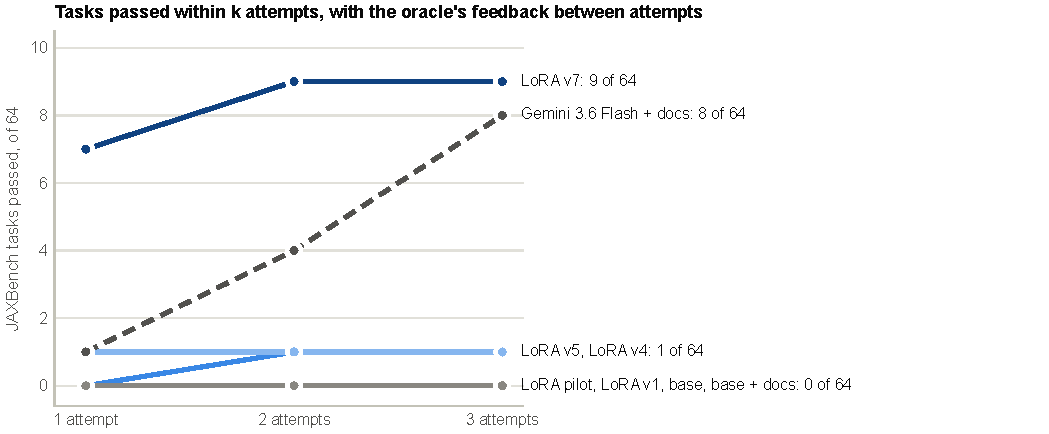
\includegraphics[width=\columnwidth]{fig11_success_vs_attempts.pdf}
\caption{Tasks passed within one, two and three attempts, over all 64 tasks. On the 58-task primary set Flash passes 7; its
eighth pass is on a task outside that set.}
\label{fig:attempts}
\end{figure}

\subsection{Correct versus fast}

The pass metric requires a kernel to be both correct and fast, and the two models fail different halves of that requirement
(Figs.~\ref{fig:speed} and \ref{fig:paired}). Flash writes a numerically correct kernel for 36 of the 58 tasks, four times as
many as the adapter's 9, and on correctness alone it is far ahead (1 task correct only for the adapter, 28 only for Flash,
$p < 10^{-6}$). But most of Flash's correct kernels are slow. The fastest correct kernel it produces per task has a median speed
of 0.54\x{} XLA, and only 7 of the 36 reach the bar.

The adapter shows the opposite profile. It is correct on only 9 tasks, but every correct kernel it writes passes, and all nine
run faster than XLA, between 1.30\x{} and 1.39\x{}. It has learned one design that is fast when it applies, and it has not
learned to fall back to a slow correct kernel when that design does not apply. Four of its passes (19k, 20k, 37k, 41k) satisfy
the oracle's second correctness rule rather than the fixed tolerance; their error equals that of XLA's own compiled reference.

\begin{figure}[t]
\centering
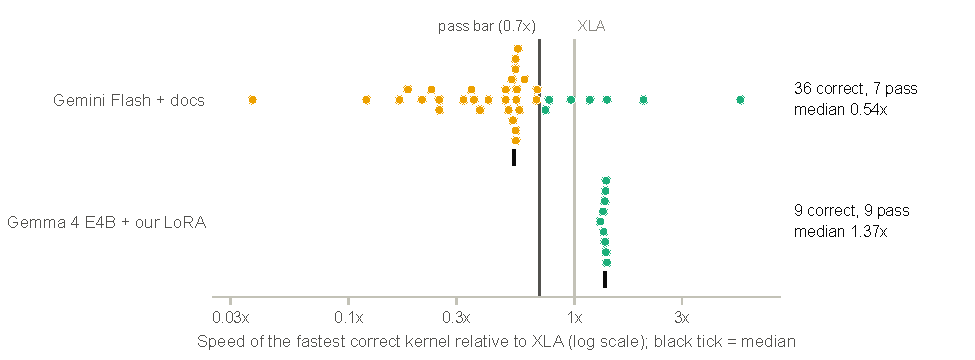
\includegraphics[width=\columnwidth]{fig16_speed_of_correct_kernels.pdf}
\caption{Speed of the fastest correct kernel per task, for every task on which each model was correct within three attempts.}
\label{fig:speed}
\end{figure}

\begin{figure}[t]
\centering
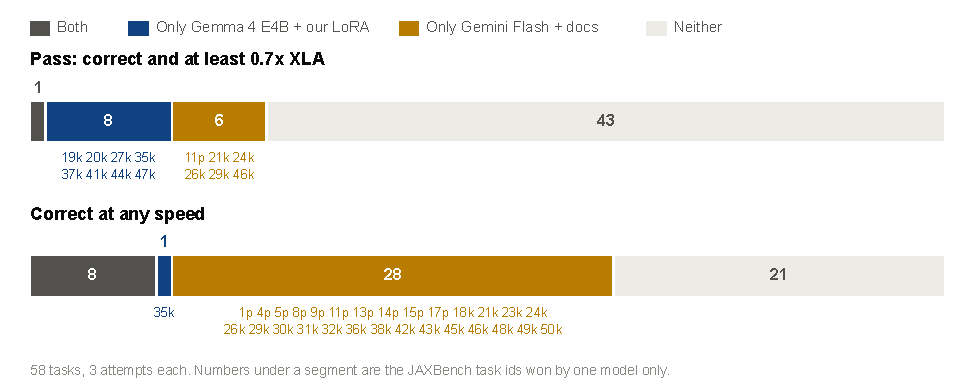
\includegraphics[width=\columnwidth]{fig17_paired_outcomes.pdf}
\caption{Paired outcomes of the adapter and Gemini Flash with documentation on the 58 primary tasks, for the pass metric (top)
and for correctness at any speed (bottom).}
\label{fig:paired}
\end{figure}

\subsection{What the adapter writes}

Eight of the nine passes are k-tasks led by a matrix multiply followed by elementwise operations; the ninth is RMSNorm. The
eight matmul kernels share one structure, shown in Fig.~\ref{fig:listing} for task 41k. The grid iterates over tiles of the
output rows, output columns and contraction axis. A float32 accumulator in VMEM is cleared on the first contraction step, each
step adds one partial product, and the last step applies the bias and activation and writes the output tile. The kernel also
raises the VMEM limit to 124~MiB. This is the tiling policy of the production-scale training rows, applied to chains of
operations that are not in the training set.

\begin{figure*}[t]
\begin{lstlisting}
def _kernel(x_ref, weight_ref, bias_ref, out_ref, acc_ref):
    k = pl.program_id(2)

    @pl.when(k == 0)
    def _zero_accumulator():
        acc_ref[...] = jnp.zeros_like(acc_ref)

    acc_ref[...] += jnp.dot(x_ref[...], weight_ref[...], preferred_element_type=jnp.float32)

    @pl.when(k == pl.num_programs(2) - 1)
    def _store_result():
        value = acc_ref[...] + bias_ref[...]
        value = jax.nn.relu(value)
        out_ref[...] = value.astype(out_ref.dtype)

def workload(x, weight, bias):
    m, k = x.shape
    n = weight.shape[1]
    tm = _tile(m, 2048, 16)
    tn = _tile(n, 2048, 128)
    tk = _tile(k, 1024, 128)
    return pl.pallas_call(
        _kernel,
        out_shape=jax.ShapeDtypeStruct((m, n), x.dtype),
        grid_spec=pltpu.PrefetchScalarGridSpec(
            num_scalar_prefetch=0,
            grid=(m // tm, n // tn, k // tk),
            in_specs=[
                pl.BlockSpec((tm, tk), lambda i, j, kk: (i, kk)),
                pl.BlockSpec((tk, tn), lambda i, j, kk: (kk, j)),
                pl.BlockSpec((tn,), lambda i, j, kk: (j,)),
            ],
            out_specs=pl.BlockSpec((tm, tn), lambda i, j, kk: (i, j)),
            scratch_shapes=[pltpu.VMEM((tm, tn), jnp.float32)],
        ),
        compiler_params=pltpu.CompilerParams(
            dimension_semantics=("parallel", "parallel", "arbitrary"),
            vmem_limit_bytes=124 * 1024 * 1024,
        ),
    )(x, weight, bias)
\end{lstlisting}
\caption{The adapter's first attempt on task 41k (a $4096 \times 8192$ input times an $8192 \times 8192$ weight, plus bias,
then ReLU), which passes at 1.37\x{} XLA. Imports and the helper \texttt{\_tile}, which picks the largest aligned tile that
divides an axis, are omitted, and the \texttt{jnp.dot} call is joined onto one line.}
\label{fig:listing}
\end{figure*}

\subsection{Where the adapter fails}

Fig.~\ref{fig:funnel} shows how far each arm gets through the oracle. The adapter's failures fall into four groups.

\emph{Compilation.} Of the 58 first attempts, 35 fail to compile, and repair does not help: across all 64 tasks, in 80 of the
81 cases where a compile failure was followed by another attempt, the next attempt also failed to compile. The oracle's
one-line feedback is enough to correct a memory layout but not a misuse of the API.

\emph{Row reductions.} Eight first attempts overflow VMEM. On repair two become passes, and six fit in memory but compute
wrong values. All six are a matmul followed by an operation over a whole output row (log-sum-exp, softmax, a row sum or a row
maximum), where the epilogue must see a complete row while the contraction axis is tiled.

\emph{Convolutions.} None of the 24 attempts on the 8 convolution-led k-tasks gets past compilation.

\emph{Production kernels.} Among the 25 p-tasks only RMSNorm passes. The others are attention variants, mixture-of-experts
routing and state-space kernels, and almost all of the adapter's attempts on them fail to compile.

\begin{figure}[t]
\centering
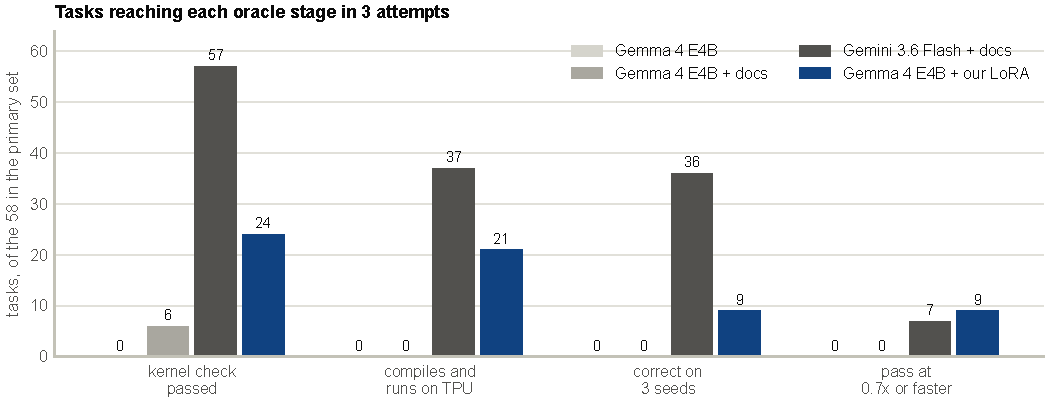
\includegraphics[width=\columnwidth]{fig12_results_funnel.pdf}
\caption{Number of primary-set tasks that reach each oracle stage within three attempts.}
\label{fig:funnel}
\end{figure}

\section{Discussion and Limitations}
\label{sec:limits}

The headline result supports a narrow claim. Fine-tuning on a few thousand verified examples moved a 4B model from never
producing a working Pallas kernel to producing fast ones for one family of tasks. The following points bound that claim, and
we consider them part of the result.

\textbf{The training data was informed by the benchmark.} No JAXBench task, reference or kernel is in the training set, and
problems with the same computation chain as a k-task were removed. However, the adapter reported here is the last of several
that we evaluated on JAXBench during development, and what we learned from earlier evaluations shaped the data. The
production-scale rows exist because an earlier adapter failed the matmul tasks, they were sized to the benchmark's matmul
scale, and 16 generated rows have exactly the input shapes of matmul tasks the adapter passes. The passed matmul tasks differ
from their nearest generated training kernel by one elementwise operation in most cases (two for 47k, four for 27k). The
correct reading of the eight matmul passes is therefore that the model applies a learned tiling design to new epilogues at
familiar shapes, and not that it designs kernels for unfamiliar problems.

\textbf{Sensitivity to near neighbours.} The contamination rule was relaxed from family level to instance level after
results of earlier adapters had been seen, which re-admitted 191 problems. If the 19 primary tasks that have a re-admitted or
same-family training neighbour are set aside, 39 tasks remain. On these the adapter passes 5, the base model 0 (exact McNemar
$p = 0.0625$) and Flash 7 (4 tasks only ours, 6 only Flash, $p = 0.75$). The direction of the effect is unchanged, but with
five discordant tasks the comparison with the base model no longer reaches the 0.05 level.

\textbf{Partial tiles.} Every template row has power-of-two sizes, so its tiles always divide the arrays, and the adapter's
kernels assume this. We re-ran the eight passed matmul tasks at two shapes absent from training, $(2048, 7168, 9216)$ and
$(3072, 7680, 8704)$. The adapter passed 3 of 8 at the first and 0 of 8 at the second. Its kernels either compute
\texttt{size // tile} grid steps and never process the remainder, or choose block sizes that the TPU rejects. The skill is
presently limited to sizes the learned tiles divide.

\textbf{The Flash reference is imperfect.} Flash differs from the adapter in model size, prompt, sampling and thinking budget,
and its control is incomplete on two tasks that only the adapter passes. On 35k its first attempt halted a TPU core; re-judged
alone it is correct at 0.22\x{} XLA, and its two repair attempts were never generated. On 19k it received two attempts instead
of three. Excluding both tasks, each model passes 7 of 56 with a 6-to-6 split of discordant tasks ($p = 1$), so the conclusion
of a tie does not depend on them.

\textbf{Testing is not verification.} Reading the training targets after training, we found 5 rows (0.2\%) whose kernels pass
the oracle through shortcuts that depend on the input distribution, such as a mean substituted for a median, or a polynomial
that is accurate only on the reference's input range. Three seeds from a fixed distribution cannot rule these out. The adapter
was trained on them; the published dataset excludes them.

\textbf{Small numbers and a single sample.} The primary set has 58 tasks, each arm contributes one chain per task, and Gemma
decodes greedily. The Wilson intervals in Table~\ref{tab:main} are wide and overlap for the adapter and Flash. Three attempts
per task is also far below the 144 used in the JAXBench paper, so none of our numbers is comparable to its reported solve
rates.

\textbf{Mixed signals in the data.} About 31\% of rows come from one generator, 15\% of targets are below the speed bar, and
most teacher kernels use the default VMEM limit while generated rows set 124~MiB. The held-out development loss (0.0002) is on
template items and measures template recall, not kernel-writing ability.

\section{Conclusion}

A 4B open model that could not write a single working Pallas kernel, with or without documentation, learned from 2,304
oracle-verified examples to write tiled matmul kernels that run 1.3\x{} to 1.4\x{} faster than XLA. On JAXBench's 58 primary
tasks with three attempts it passes 9, a significant improvement over the base model's 0 and a statistical tie with Gemini
Flash given documentation. The tie hides a clear difference in kind: Flash is correct four times as often and usually slow,
and the adapter is rarely correct but fast whenever it is. The adapter's competence is confined to the matmul family at
sizes its tiles divide, most of its failures never compile, and the training data was shaped by the benchmark it is scored
on. The next steps follow directly from the failures: training rows with partial tiles, rows that teach whole-row reductions
under a tiled contraction, and feedback that explains compile errors rather than reporting them.

\section*{Reproducibility}

Code, data and results are in the repository \texttt{Art4v/gemma-hackathon-research}. The oracle is in \texttt{oracle/}. The
release \texttt{dataset-final} contains the training file as trained (2,304 rows), the published file without the five
shortcut rows (2,299 rows), the development set, a datasheet \cite{datasheets} and checksums. The raw generations and verdicts of every arm are
in \texttt{paper/data/runs/}, and \texttt{paper/analysis/jaxbench.py} recomputes every number in Tables~\ref{tab:main} and
\ref{tab:mcnemar} from them using only the Python standard library.

\begin{thebibliography}{00}
\bibitem{jax} J. Bradbury \emph{et al.}, ``JAX: composable transformations of Python+NumPy programs,'' 2018. [Online].
Available: \url{http://github.com/jax-ml/jax}
\bibitem{pallas} The JAX authors, ``Pallas: a JAX kernel language,'' JAX documentation.
\bibitem{jaxbench} JAXBench authors, ``JAXBench,'' 2026. [Full reference to be added.]
\bibitem{kernelbench} A. Ouyang \emph{et al.}, ``KernelBench: Can LLMs write efficient GPU kernels?'' in \emph{Proc. ICML}, 2025.
\bibitem{kbverified} ``KernelBench-Verified.'' [Full reference to be added.]
\bibitem{kernelllm} Meta, ``KernelLLM,'' model release, 2025.
\bibitem{autotriton} S. Li \emph{et al.}, ``AutoTriton: Automatic Triton programming with reinforcement learning in LLMs,''
arXiv preprint, 2025.
\bibitem{tritonrl} ``TritonRL,'' arXiv preprint, 2025. [Full reference to be added.]
\bibitem{drkernel} ``Dr.~Kernel.'' [Full reference to be added.]
\bibitem{kevin} C. Baronio \emph{et al.}, ``Kevin: Multi-turn RL for generating CUDA kernels,'' arXiv preprint, 2025.
\bibitem{gemma4} Google DeepMind, ``Gemma 4,'' model release, 2026. [Full reference to be added.]
\bibitem{kimi} Moonshot AI, ``Kimi K3.1,'' model release, 2026. [Full reference to be added.]
\bibitem{lora} E. J. Hu \emph{et al.}, ``LoRA: Low-rank adaptation of large language models,'' in \emph{Proc. ICLR}, 2022.
\bibitem{mcnemar} Q. McNemar, ``Note on the sampling error of the difference between correlated proportions or percentages,''
\emph{Psychometrika}, vol. 12, no. 2, pp. 153--157, 1947.
\bibitem{holm} S. Holm, ``A simple sequentially rejective multiple test procedure,'' \emph{Scand. J. Statist.}, vol. 6, no. 2,
pp. 65--70, 1979.
\bibitem{wilson} E. B. Wilson, ``Probable inference, the law of succession, and statistical inference,'' \emph{J. Amer.
Statist. Assoc.}, vol. 22, no. 158, pp. 209--212, 1927.
\bibitem{mlir} C. Lattner \emph{et al.}, ``MLIR: Scaling compiler infrastructure for domain specific computation,'' in \emph{Proc. CGO}, 2021.
\bibitem{halide} J. Ragan-Kelley \emph{et al.}, ``Halide: A language and compiler for optimizing parallelism, locality, and
recomputation in image processing pipelines,'' in \emph{Proc. PLDI}, 2013.
\bibitem{tvm} T. Chen \emph{et al.}, ``TVM: An automated end-to-end optimizing compiler for deep learning,'' in \emph{Proc. OSDI}, 2018.
\bibitem{ansor} L. Zheng \emph{et al.}, ``Ansor: Generating high-performance tensor programs for deep learning,'' in \emph{Proc. OSDI}, 2020.
\bibitem{tpu} N. P. Jouppi \emph{et al.}, ``In-datacenter performance analysis of a tensor processing unit,'' in \emph{Proc. ISCA}, 2017.
\bibitem{triton} P. Tillet, H. T. Kung, and D. Cox, ``Triton: An intermediate language and compiler for tiled neural network
computations,'' in \emph{Proc. MAPL}, 2019.
\bibitem{codex} M. Chen \emph{et al.}, ``Evaluating large language models trained on code,'' arXiv:2107.03374, 2021.
\bibitem{alphacode} Y. Li \emph{et al.}, ``Competition-level code generation with AlphaCode,'' \emph{Science}, vol. 378, no. 6624, pp. 1092--1097, 2022.
\bibitem{codellama} B. Rozi\`ere \emph{et al.}, ``Code Llama: Open foundation models for code,'' arXiv:2308.12950, 2023.
\bibitem{starcoder} R. Li \emph{et al.}, ``StarCoder: May the source be with you!'' arXiv:2305.06161, 2023.
\bibitem{distill} G. Hinton, O. Vinyals, and J. Dean, ``Distilling the knowledge in a neural network,'' arXiv:1503.02531, 2015.
\bibitem{pie} A. Shypula \emph{et al.}, ``Learning performance-improving code edits,'' in \emph{Proc. ICLR}, 2024.
\bibitem{swebench} C. E. Jimenez \emph{et al.}, ``SWE-bench: Can language models resolve real-world GitHub issues?'' in \emph{Proc. ICLR}, 2024.
\bibitem{alphadev} D. J. Mankowitz \emph{et al.}, ``Faster sorting algorithms discovered using deep reinforcement learning,''
\emph{Nature}, vol. 618, pp. 257--263, 2023.
\bibitem{qlora} T. Dettmers, A. Pagnoni, A. Holtzman, and L. Zettlemoyer, ``QLoRA: Efficient finetuning of quantized LLMs,'' in \emph{Proc. NeurIPS}, 2023.
\bibitem{qat} B. Jacob \emph{et al.}, ``Quantization and training of neural networks for efficient integer-arithmetic-only
inference,'' in \emph{Proc. CVPR}, 2018.
\bibitem{selfdebug} X. Chen, M. Lin, N. Sch\"arli, and D. Zhou, ``Teaching large language models to self-debug,'' in \emph{Proc. ICLR}, 2024.
\bibitem{adamw} I. Loshchilov and F. Hutter, ``Decoupled weight decay regularization,'' in \emph{Proc. ICLR}, 2019.
\bibitem{dietterich} T. G. Dietterich, ``Approximate statistical tests for comparing supervised classification learning
algorithms,'' \emph{Neural Comput.}, vol. 10, no. 7, pp. 1895--1923, 1998.
\bibitem{datasheets} T. Gebru \emph{et al.}, ``Datasheets for datasets,'' \emph{Commun. ACM}, vol. 64, no. 12, pp. 86--92, 2021.
\end{thebibliography}

\end{document}
